\section{Appendix}



\subsection{Visible Comparison Examples}  \label{sec:appedix_visible_example}
\begin{figure}[H]
    \centering
    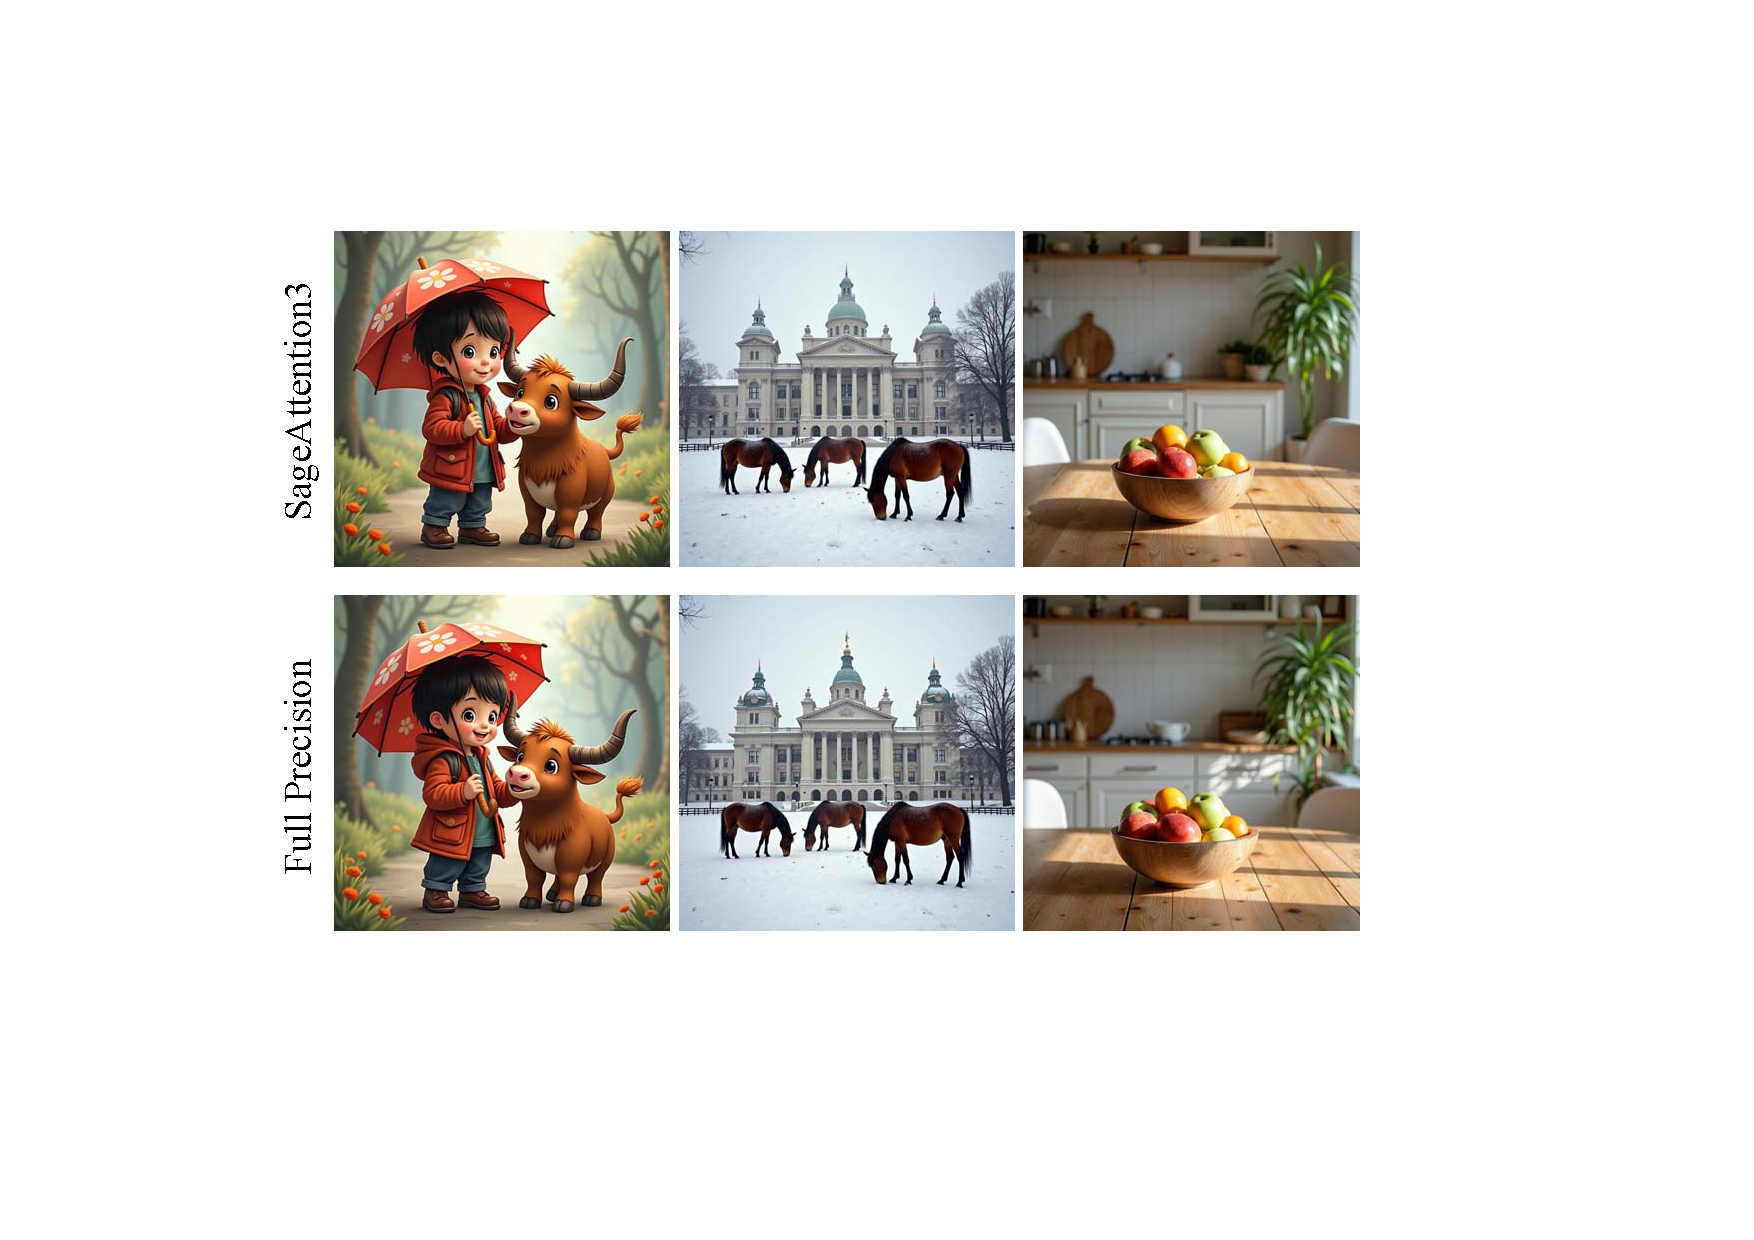
\includegraphics[width=.75\columnwidth]{src/figs/sd.pdf} 
    \caption{Visible examples of image generation on \texttt{Stable-Diffusion3.5}.}
    \label{fig:sd_visual} 
\end{figure}

\begin{figure}[H]
    \centering
    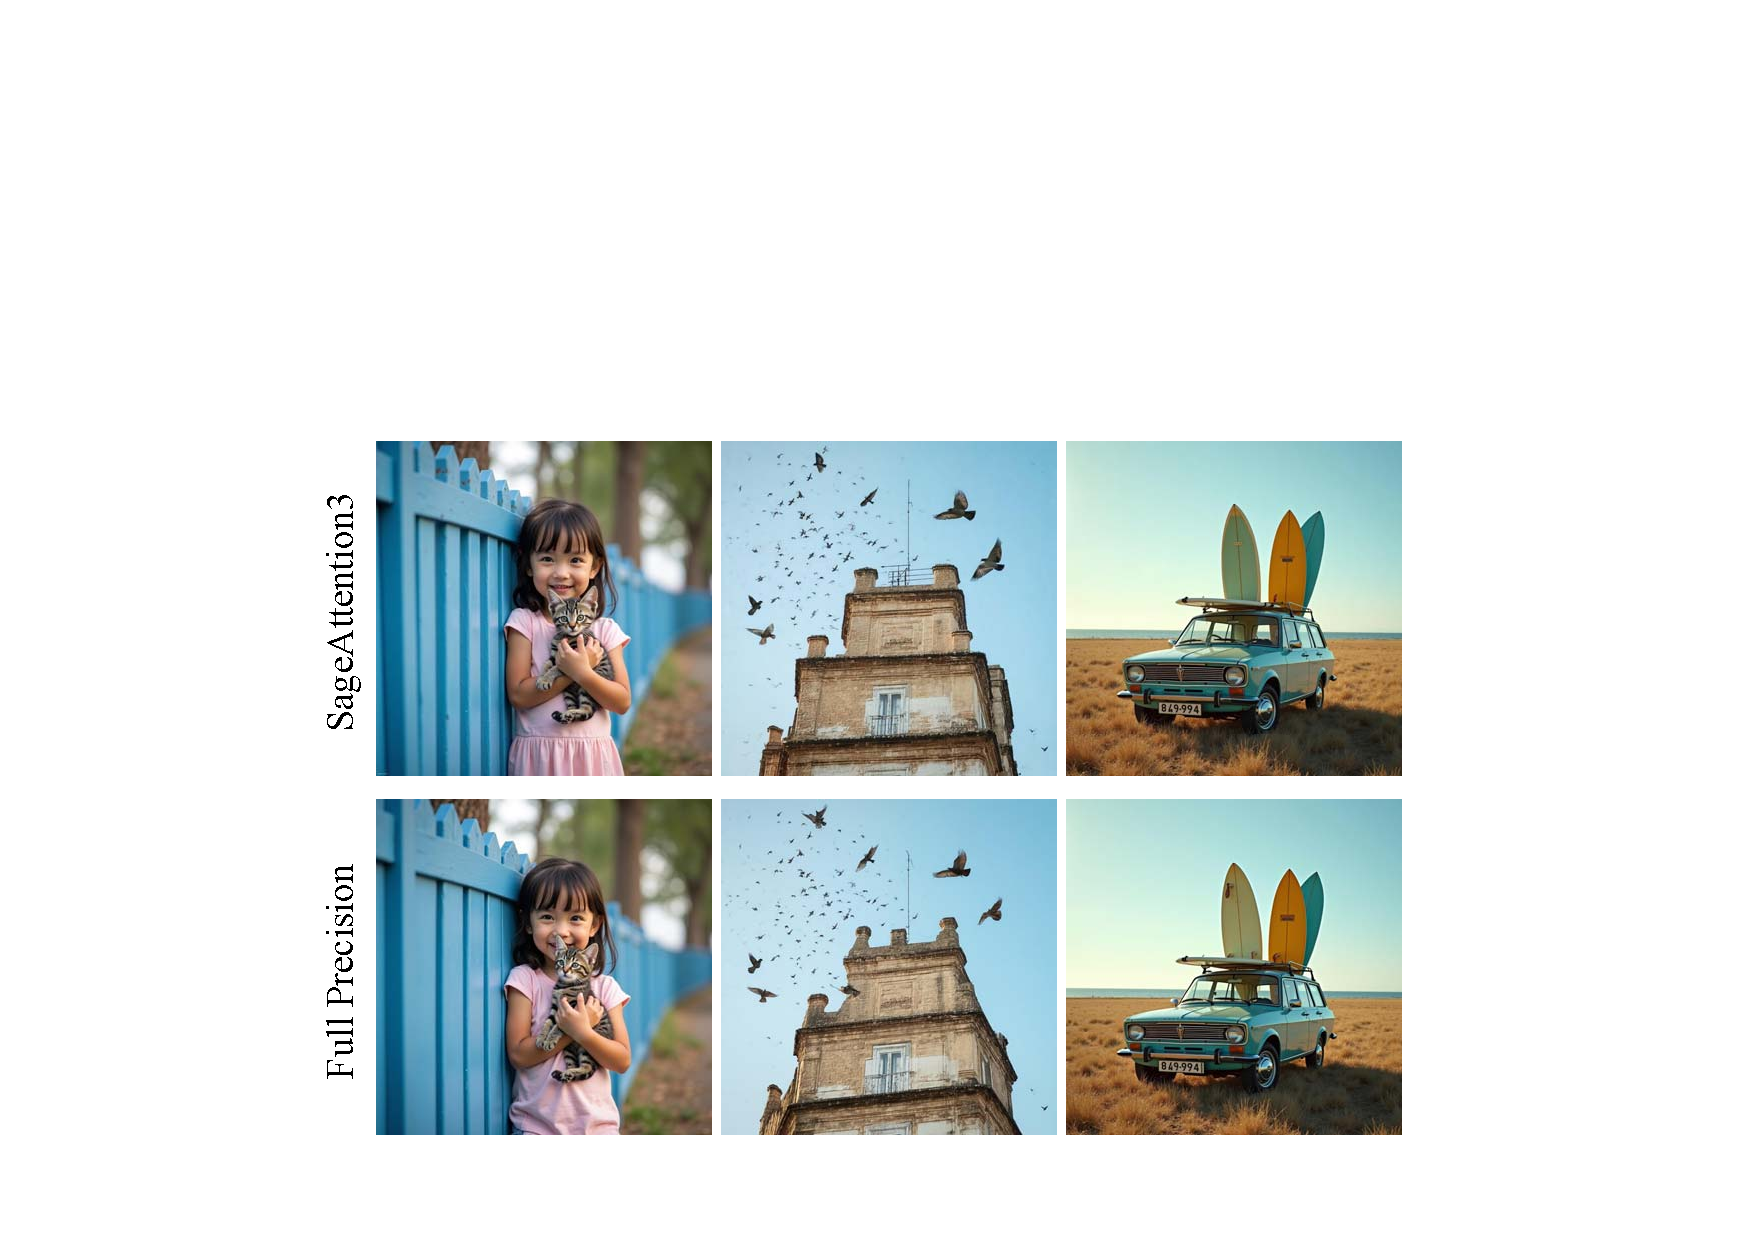
\includegraphics[width=.75\columnwidth]{src/figs/flux.pdf} 
    \caption{Visible examples of image generation on \texttt{Flux}.}
    \label{fig:flux_visual} 
\end{figure}

\begin{figure}[H]
    \centering
    \begin{subfigure}[b]{0.3\textwidth}
        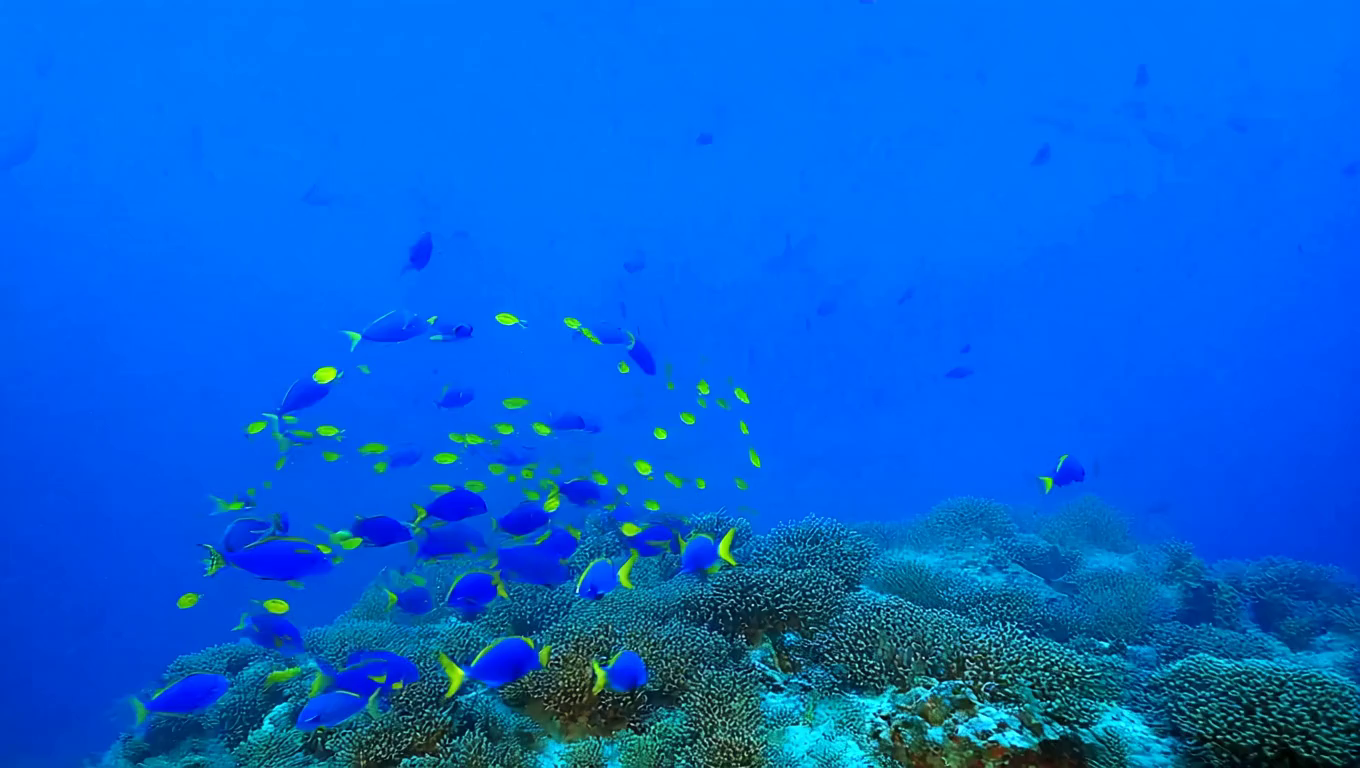
\includegraphics[width=\textwidth]{src/figs/scale_ablation/CogVideoX-5B.png}
        \caption{Full-Precision}
        \label{fig:a}
    \end{subfigure}
    \hfill
    \begin{subfigure}[b]{0.3\textwidth}
        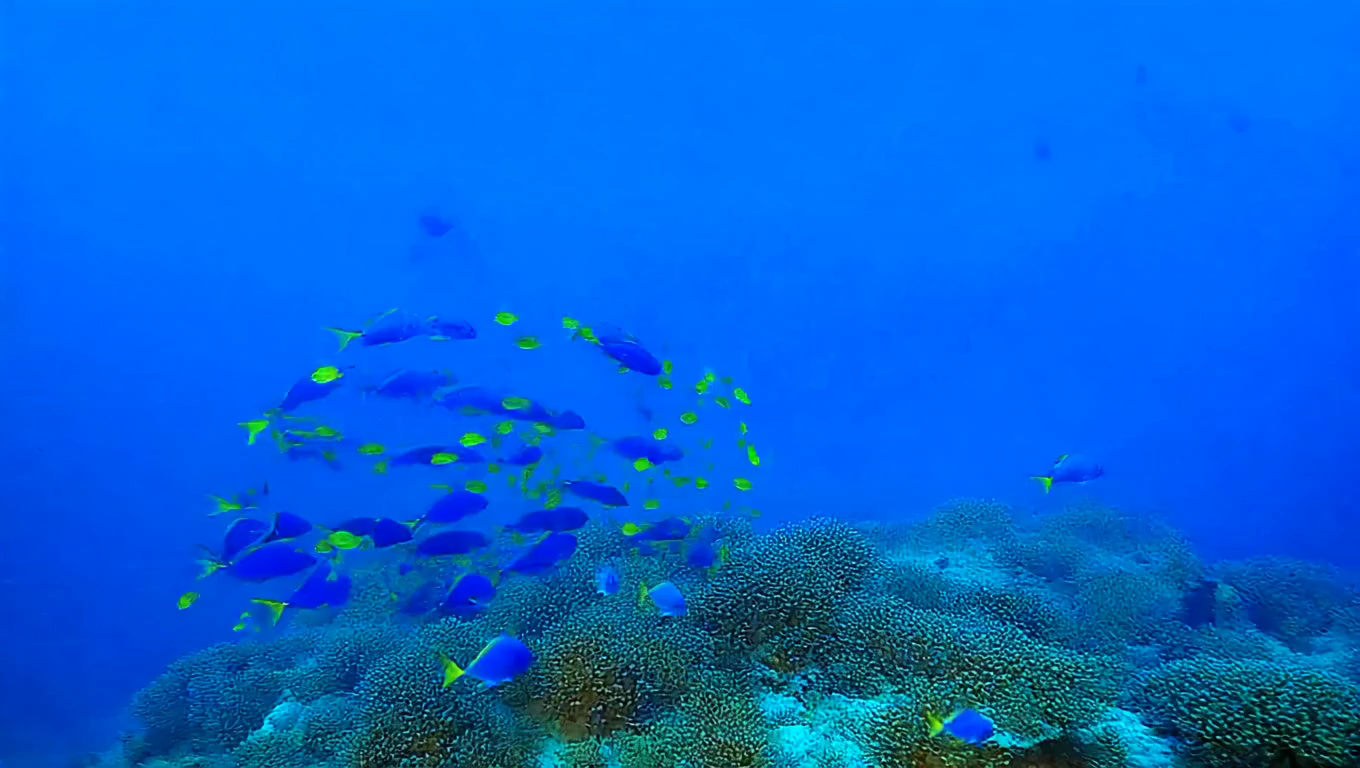
\includegraphics[width=\textwidth]{src/figs/scale_ablation/sage3.png}
        \caption{Two-level quantization}
        \label{fig:b}
    \end{subfigure}
    \hfill
    \begin{subfigure}[b]{0.3\textwidth}
        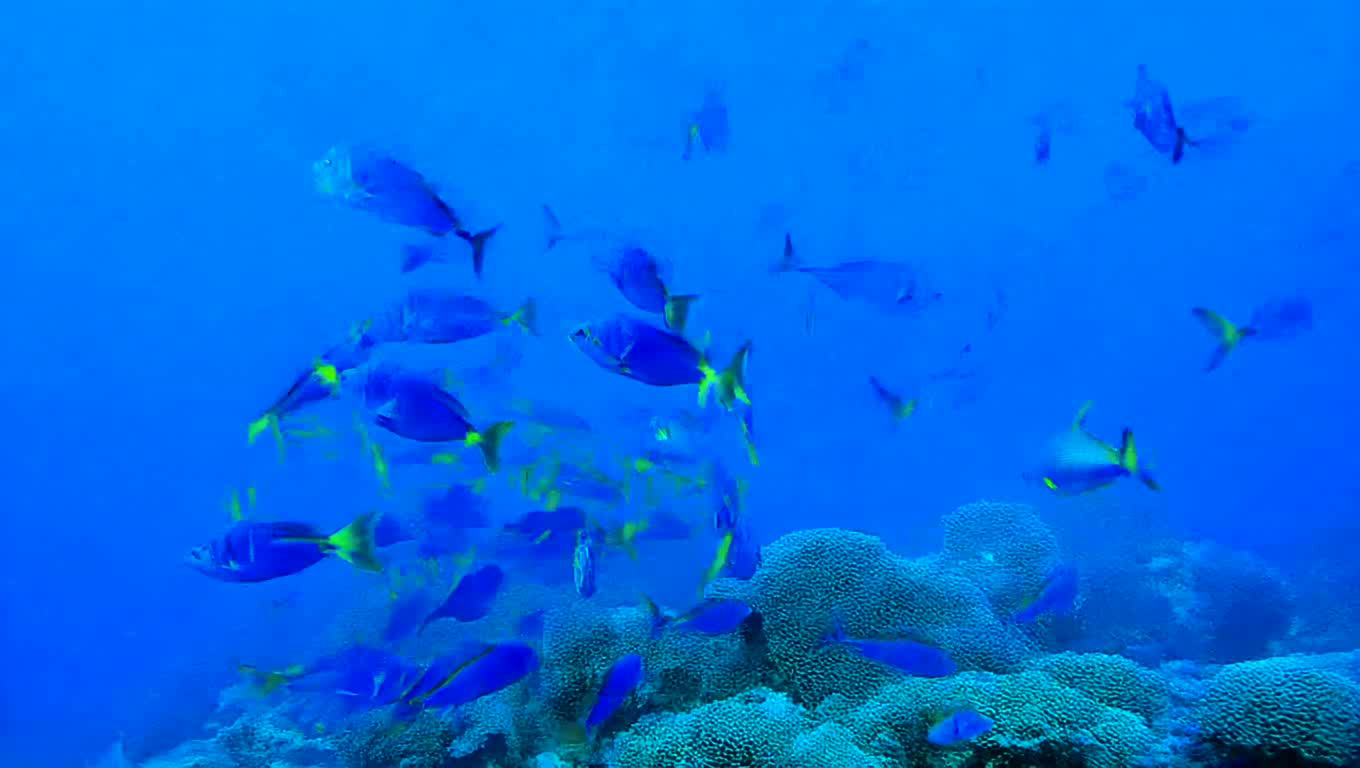
\includegraphics[width=\textwidth]{src/figs/scale_ablation/sage3_no_scale.png}
        \caption{Direct quantization}
        \label{fig:c}
    \end{subfigure}
    \caption{Visual comparison of different scale strategies for $\widetilde \vP$ from \texttt{CogVideoX}.}
    \label{fig:scale_ablation}
\end{figure}


\begin{figure}[H]
    \centering
    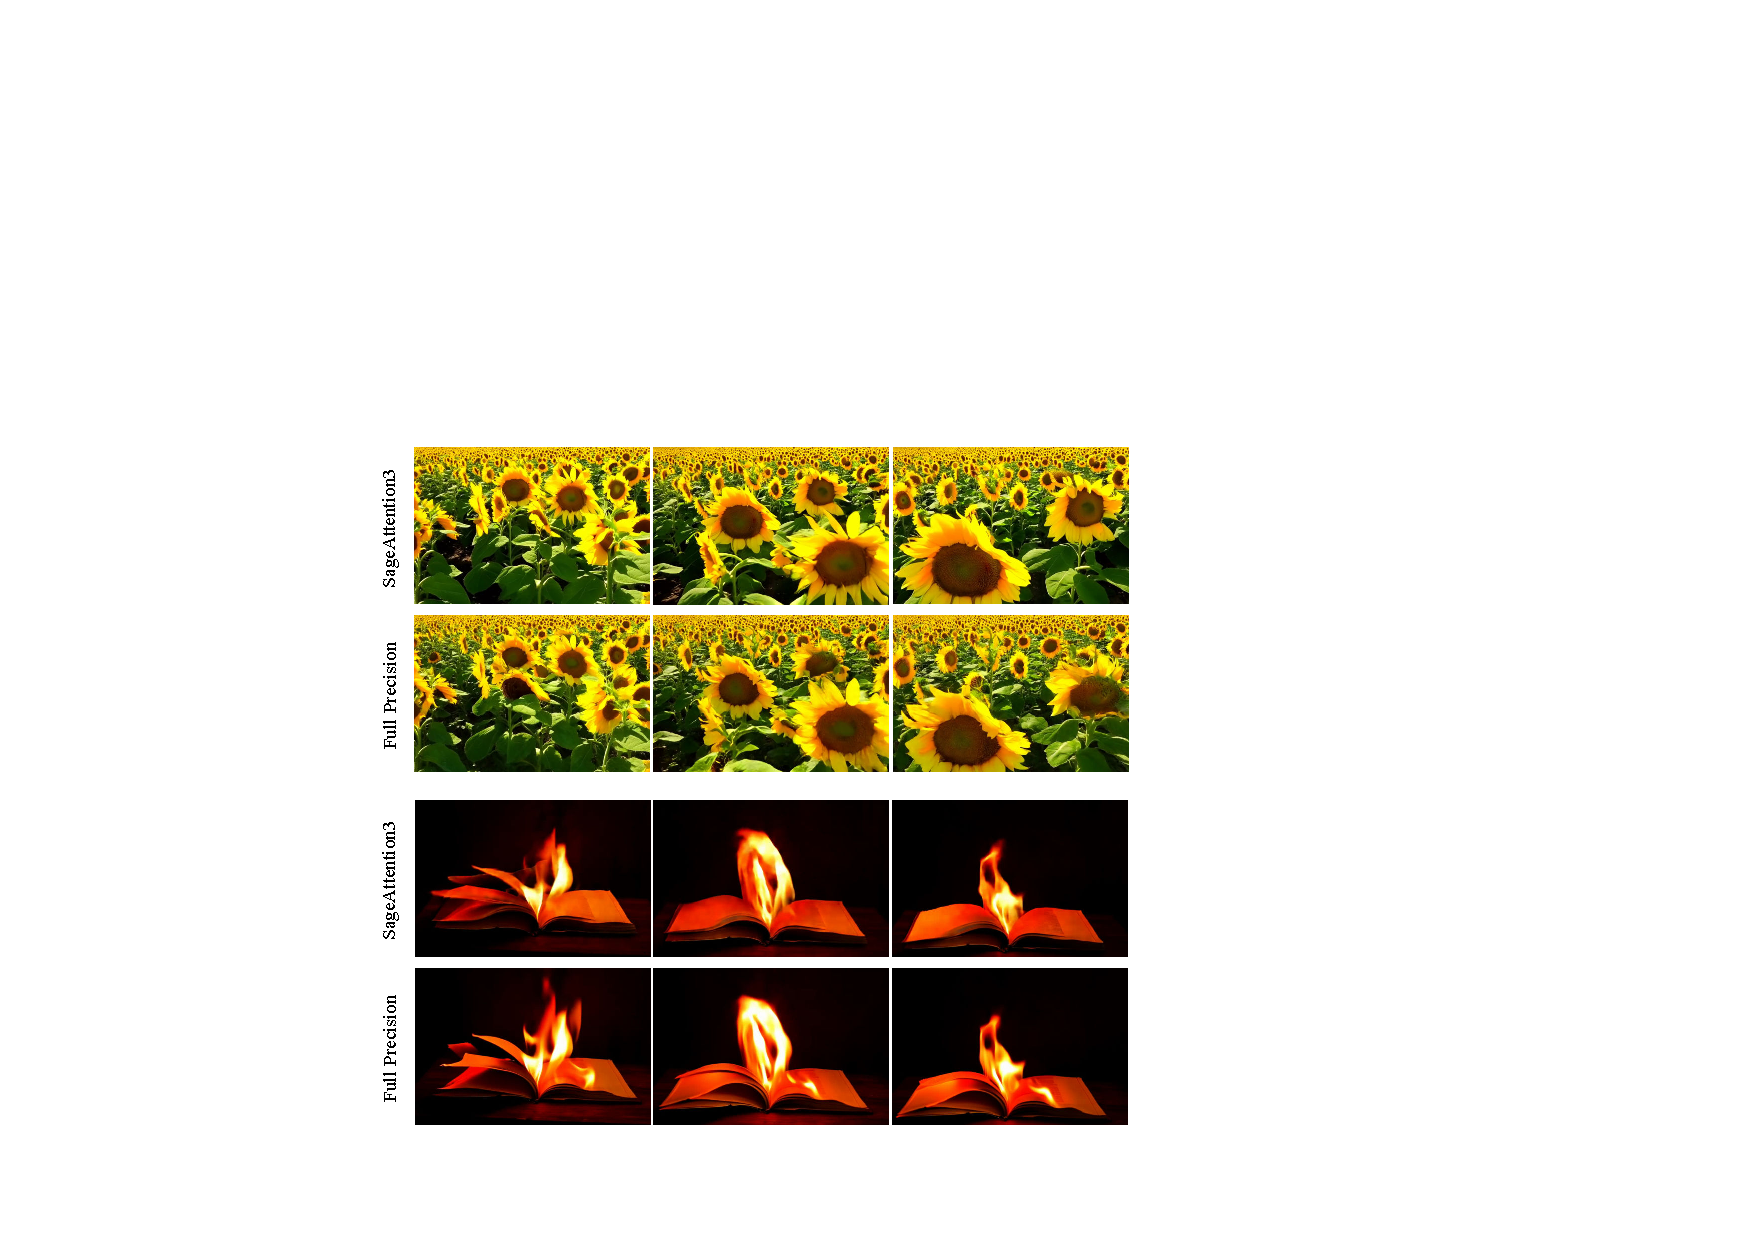
\includegraphics[width=.885\columnwidth]{src/figs/cog.pdf} 
    \vspace{-.25em}
    \caption{Visible examples of video generation on \texttt{CogVideoX}.}
    \vspace{-1.5em}
    \label{fig:cog_visual} 
\end{figure}

\begin{figure}[H]
    \centering
    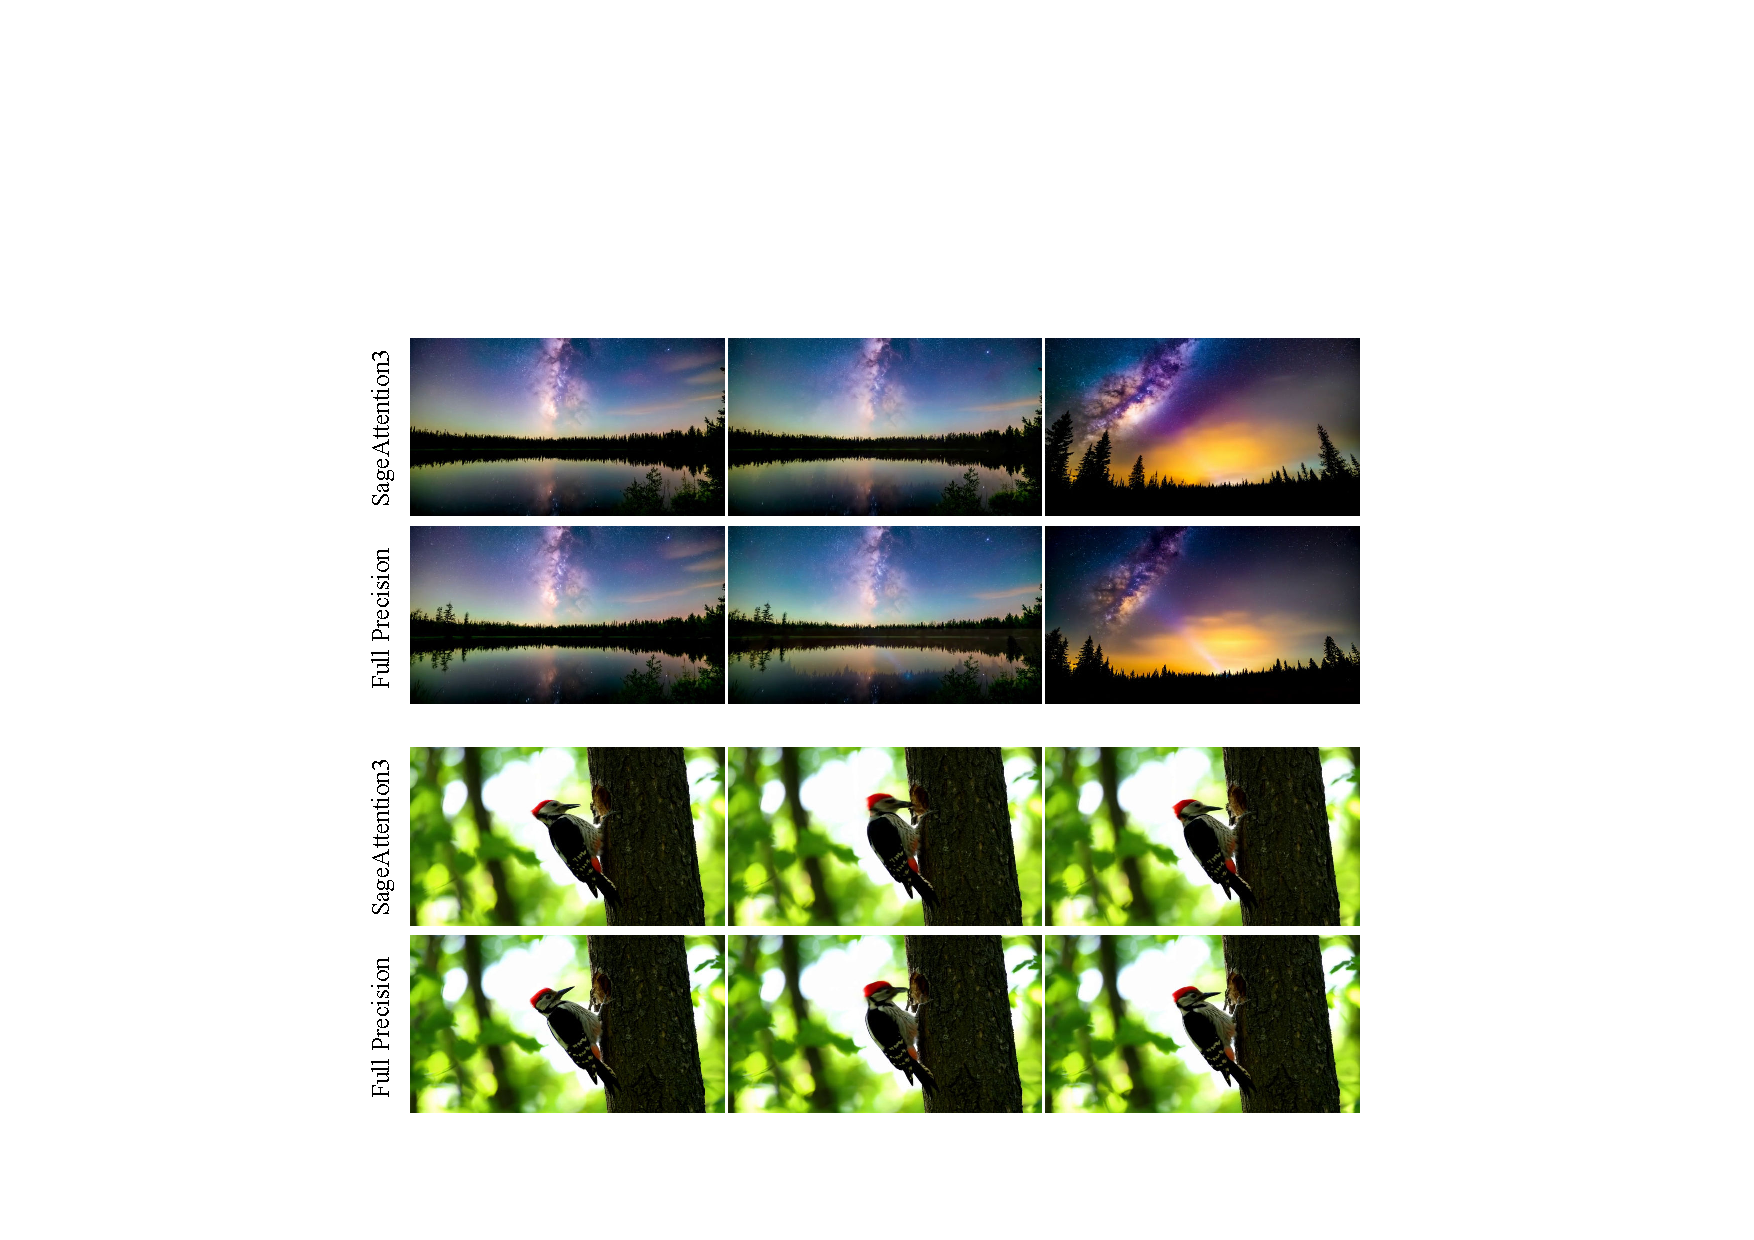
\includegraphics[width=.885\columnwidth]{src/figs/hunyuan.pdf} 
    \vspace{-.25em}
    \caption{Visible examples of video generation on \texttt{HunyuanVideo}.}
    \label{fig:hunyuan_visual} 
\end{figure}


Fig.~\ref{fig:sd_visual} and Fig.~\ref{fig:flux_visual} show additional visual comparison examples of image generation tasks. Fig.~\ref{fig:cog_visual} and Fig.~\ref{fig:hunyuan_visual} show more visual comparison examples of video generation tasks. 


\subsection{Additional Kernel Speed Comparison}  \label{sec:appedix_kernel_speed}

Fig.~\ref{fig:sage_train_fwd_h128_speed} and Fig.~\ref{fig:sage_train_fwd_h64_speed} show the forward kernel speed of \texttt{SageBwd}. Fig.~\ref{fig:sage_train_bwd_h128_speed} and Fig.~\ref{fig:sage_train_bwd_h64_speed} show the backward kernel speed of \texttt{SageBwd}. \texttt{SageBwd} achieved a \textbf{2x} speed up than FlashAttention in the forward propagation. \texttt{SageBwd} achieved a 1.2\textasciitilde\textbf{1.6x} speed up than FlashAttention in the backward propagation.
 \begin{figure}[H]
  \centering
  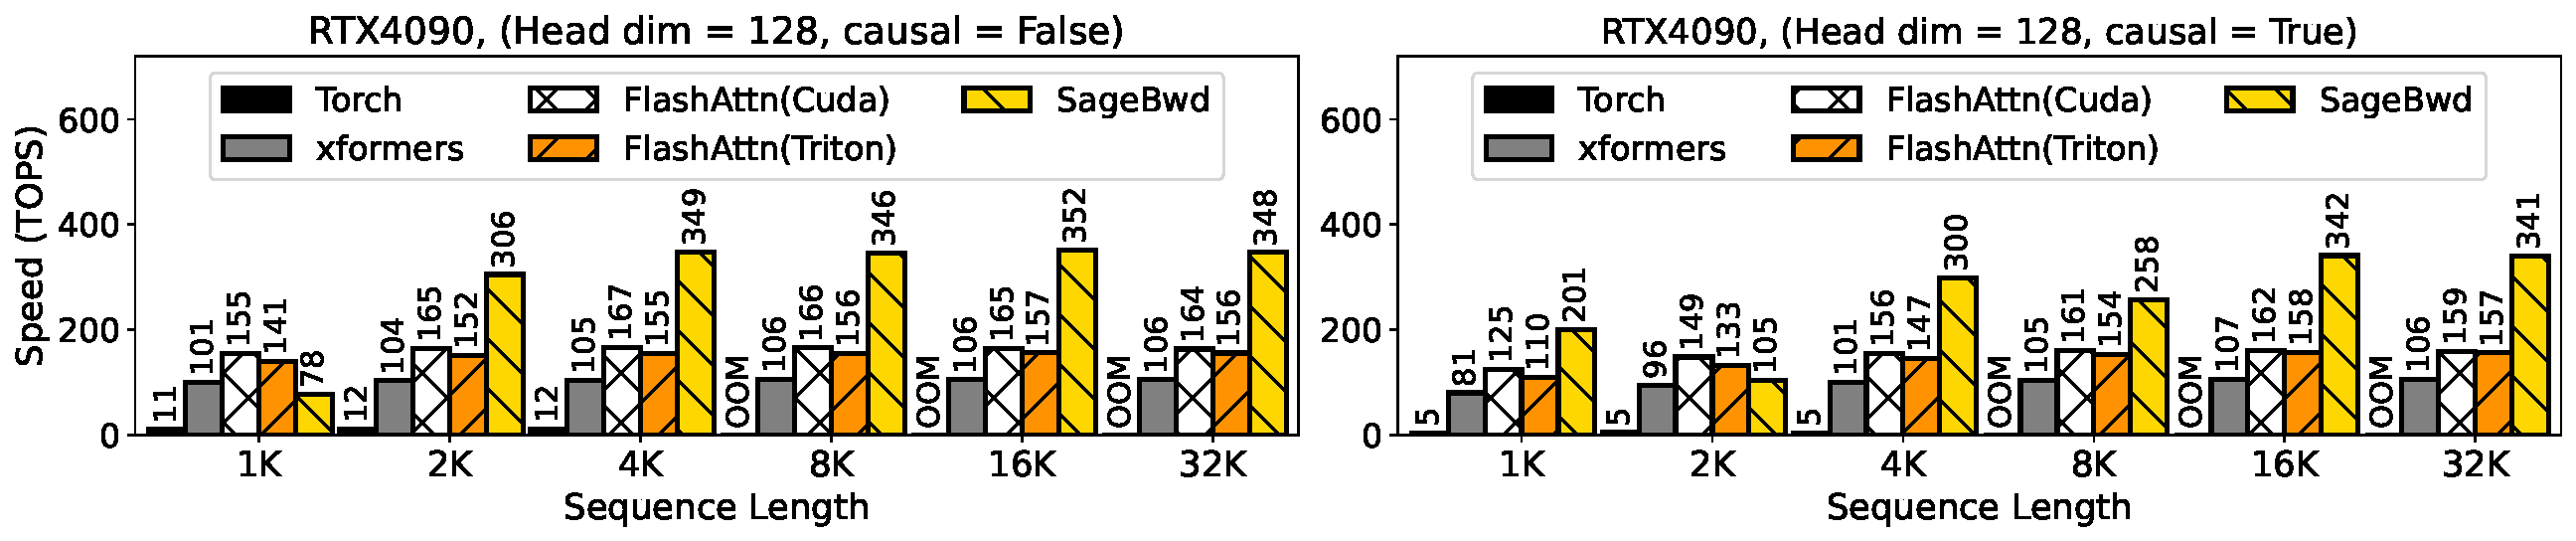
\includegraphics[width=\columnwidth]{src/figs/sage_attn_train_fwd_hd128_baselines_kernel_flops.pdf} 
  \vspace{-1em}
  \caption{Forward speed comparison between \texttt{SageBwd} and Baselines (\texttt{RTX4090}, headim=128).}
  \label{fig:sage_train_fwd_h128_speed} 
\end{figure}
\begin{figure}[H]
  \centering
  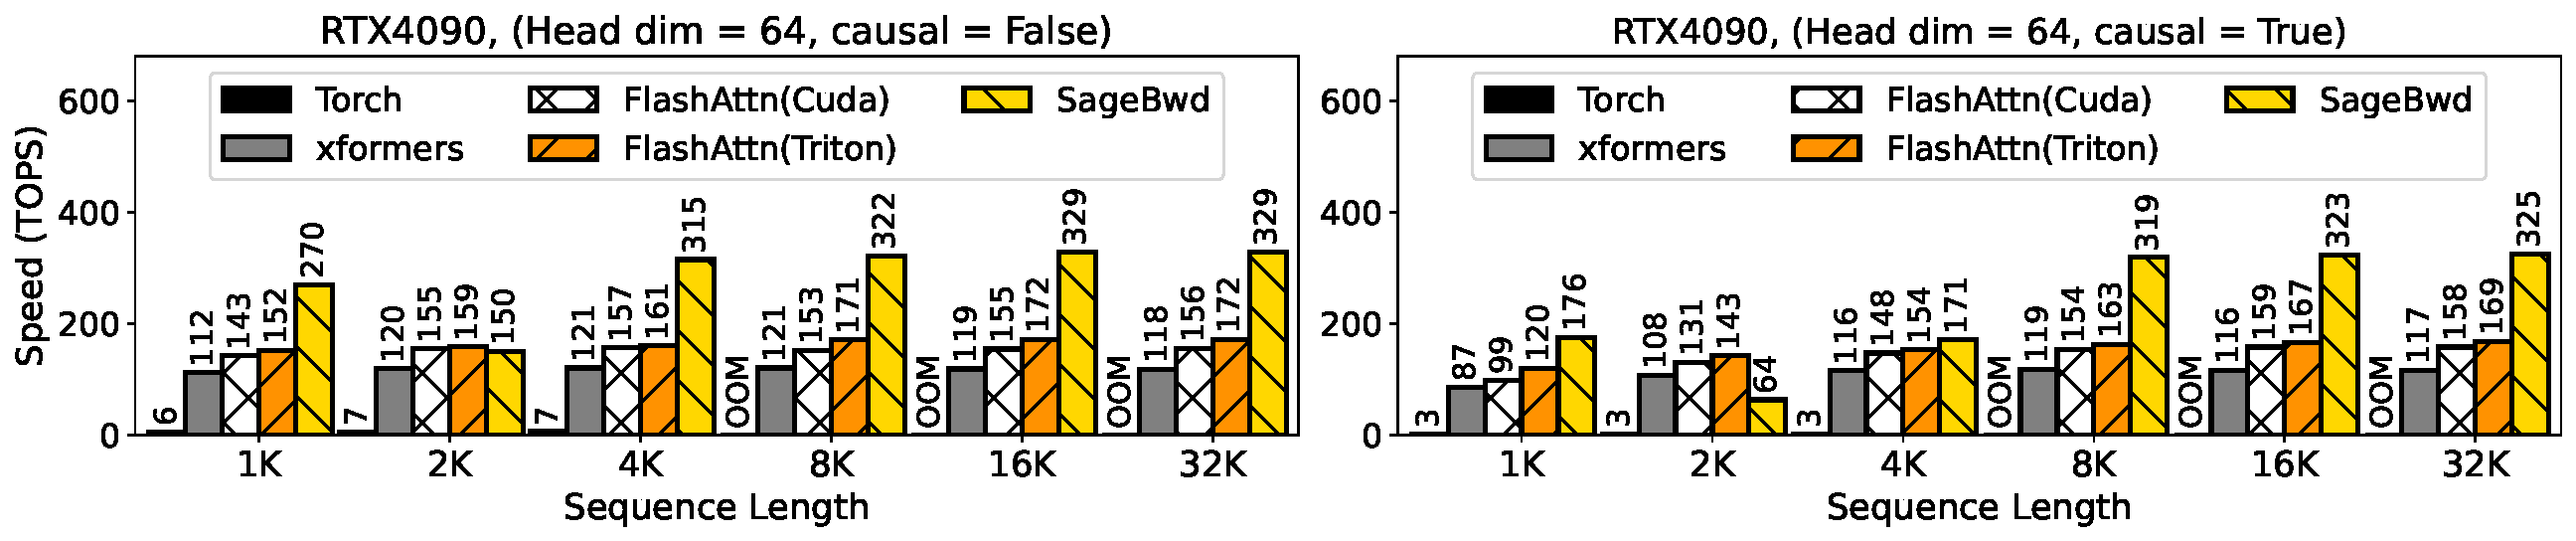
\includegraphics[width=\columnwidth]{src/figs/sage_attn_train_fwd_hd64_baselines_kernel_flops.pdf} 
  \vspace{-1em}
  \caption{Forward speed comparison between \texttt{SageBwd} and Baselines (\texttt{RTX4090}, headim=64).}
  \label{fig:sage_train_fwd_h64_speed} 
\end{figure}

\begin{figure}[H]
  \centering
  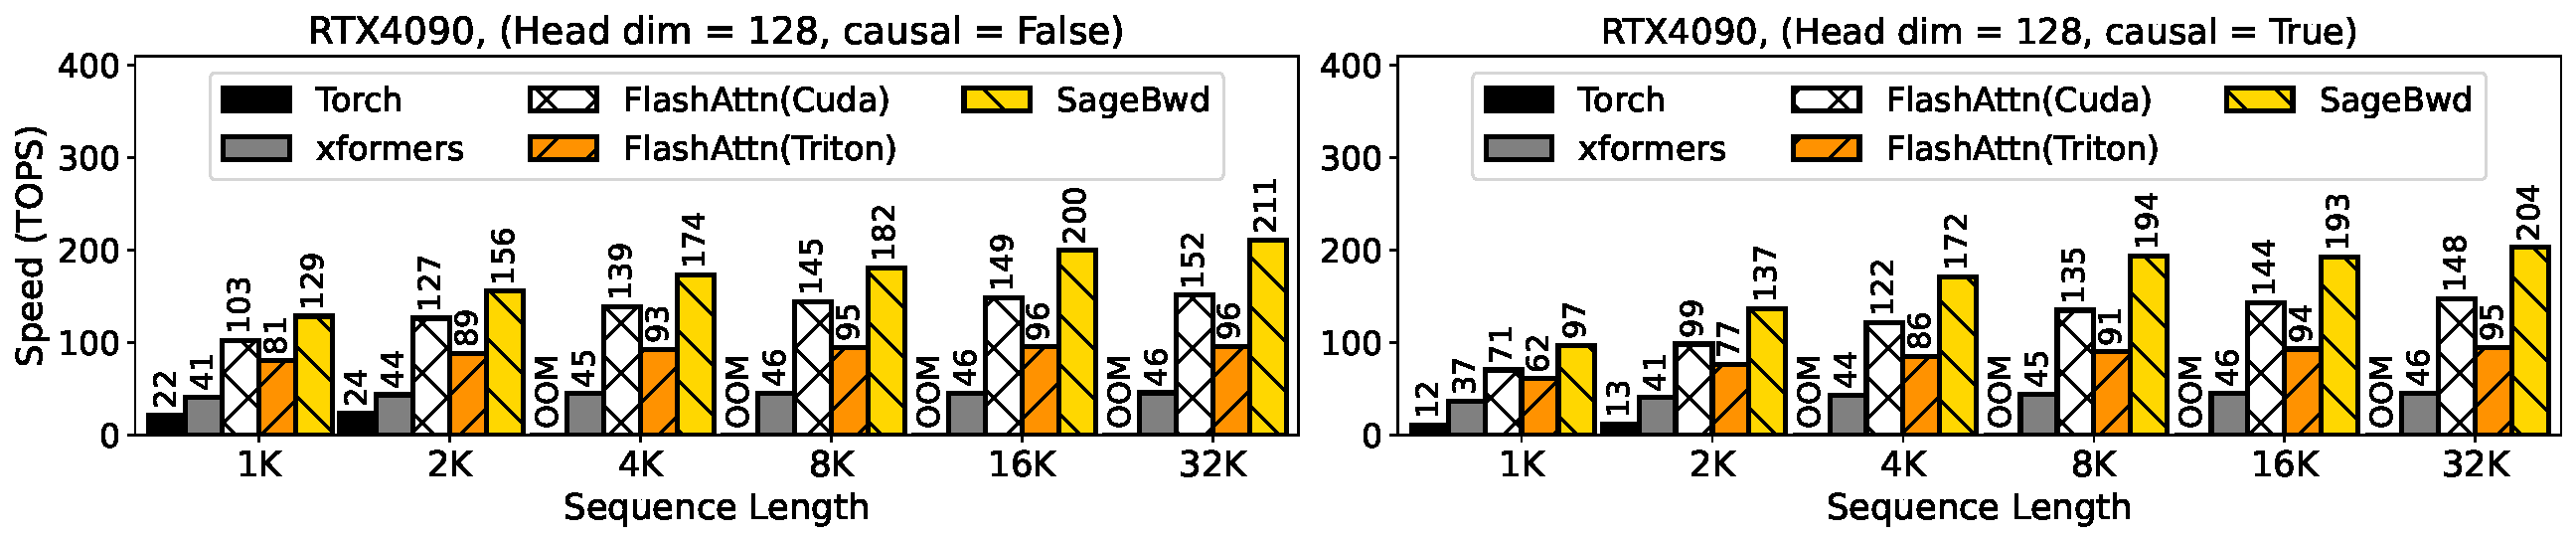
\includegraphics[width=\columnwidth]{src/figs/sage_attn_train_bwd_hd128_baselines_kernel_flops.pdf} 
  \vspace{-1em}
  \caption{Backward speed comparison between \texttt{SageBwd} and Baselines (\texttt{RTX4090}, headim=128).}
  \label{fig:sage_train_bwd_h128_speed} 
\end{figure}
\begin{figure}[H]
    \centering
    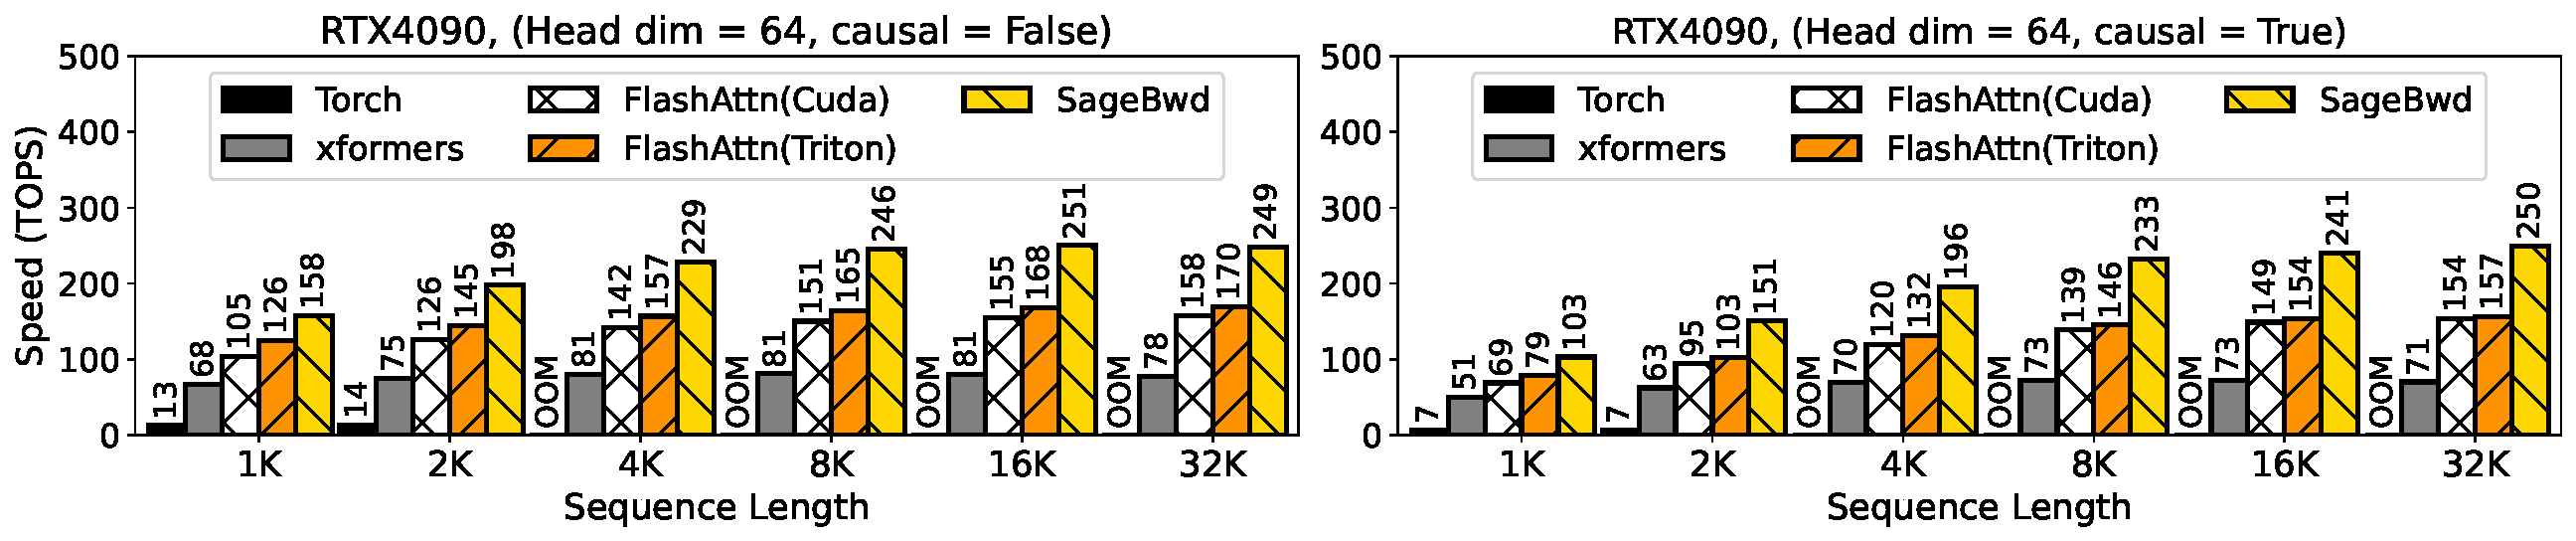
\includegraphics[width=\columnwidth]{src/figs/sage_attn_train_bwd_hd64_baselines_kernel_flops.pdf} 
    \vspace{-1em}
    \caption{Backward speed comparison between \texttt{SageBwd} and Baselines (\texttt{RTX4090}, headim=64).}
    \label{fig:sage_train_bwd_h64_speed} 
\end{figure}


\subsection{Datasets, Metrics, and Hyperparameters}  \label{sec:exp_dataset_metrics}
\noindent \noindent\textbf{Datasets.}   
Text-to-video models are evaluated using the open-sora~\citep{opensora} prompt sets.
Text-to-image models are assessed on COCO annotations~\citep{lin2014microsoft}.
Language models are evaluated on GSM8K~\citep{cobbe2021gsm8k}, DROP~\citep{Dua2019DROP}, MMLU~\citep{MMLU}, and HELLASWAG~\citep{zellers2019hellaswag} datasets.


\noindent \noindent\textbf{End-to-end metrics.}   
For text-to-text models, we use Accuracy (Acc.) and F1-Score (F1).
For text-to-video models, we evaluate the quality of generated videos on five metrics: CLIPSIM and CLIP-Temp (CLIP-T)~\cite{liu2024evalcrafter} to measure the text-video alignment; (VQA-a) and (VQA-t) to assess the video aesthetic and technical quality, respectively; and Flow-score (FScore) for temporal consistency~\cite{wu2023exploring}. 
For text-to-image models, generated images are evaluated in three aspects: FID~\cite{heusel2017gans} and sFID~\cite{salimans2016improved} for fidelity evaluation, \textit{Clipscore} (CLIP)~\cite{hessel2021clipscore} for text-image alignment, and \textit{ImageReward} (IR)~\cite{xu2024imagereward} for human preference.

\noindent\textbf{Accuracy metrics.} We use three metrics to assess the accuracy of quantized attention output $O'$ compared to attention output in full-precision $O$: First, we flatten $O'$ and $O$ into vectors in the shape of $1\times n$. Then, Cosine similarity: $CosSim=\sum OO' / \smash{\sqrt{\sum O^2}} \smash{\sqrt{\sum O'^2}}$, Relative L1 distance: $L1=\sum |O - O'| / \sum |O|$, Root mean square error: $RMSE=\sqrt{(1/n) \sum (O - O')^2}$.

\textbf{Hyperparameters.} 
For pretraining tasks, we use a 400M model with a hidden size of 1024, 20 layers, an intermediate size of 3072, and 16 attention heads. The training uses a learning rate of 1e-3 with linear decay over 1000 warmup steps, and each step processes 2M tokens.
For finetuning tasks, we train for 700 steps using a learning rate of 3e-5 with linear decay and 100 warmup steps with a batch size of 32 on GSM8K dataset and 128 on MMLU, DROP, and HELLASWAG datasets.

\begin{figure}[H]
    \centering
    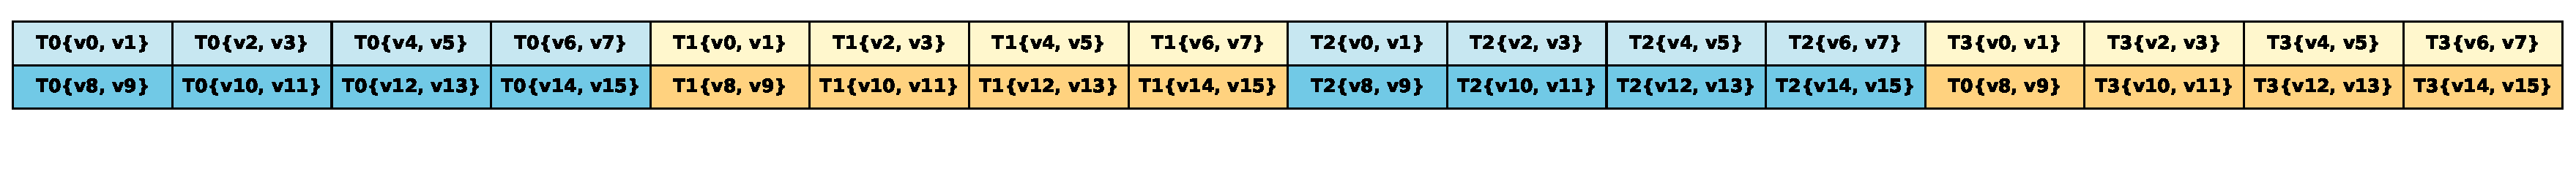
\includegraphics[width=1\columnwidth]{src/figs/fp4input.pdf} 
    \vspace{-1em}
    \caption{\texttt{FP4} operand A register layout - rows 0 and 8, thread 0-3, entries 0-15.}
    \label{fig:input_layout} 
\end{figure}
\begin{figure}[H]
    \centering
    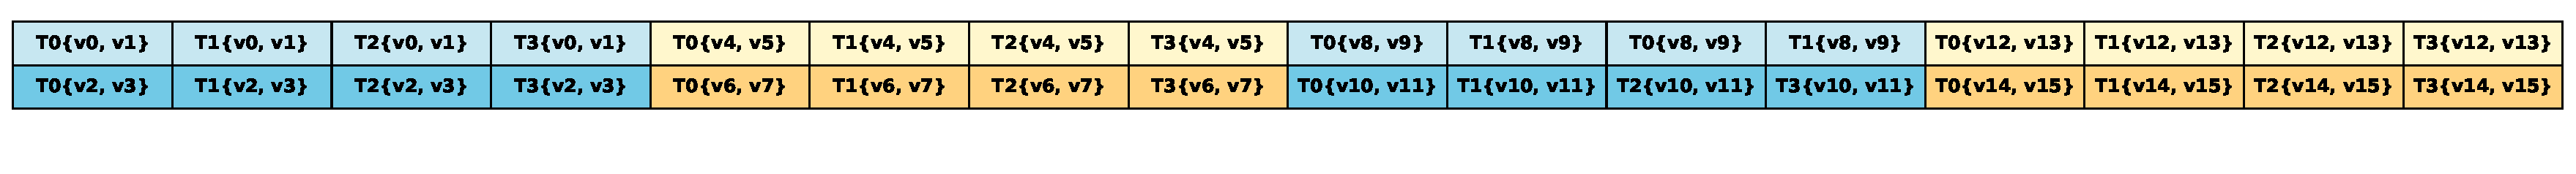
\includegraphics[width=1\columnwidth]{src/figs/ori_fp32.pdf} 
    \vspace{-1em}
    \caption{\texttt{FP32} accumulator register layout - rows 0 and 8, thread 0-3, entries 0-15.}
    \label{fig:ori_fp32_layout} 
\end{figure}
\begin{figure}[H]
    \centering
    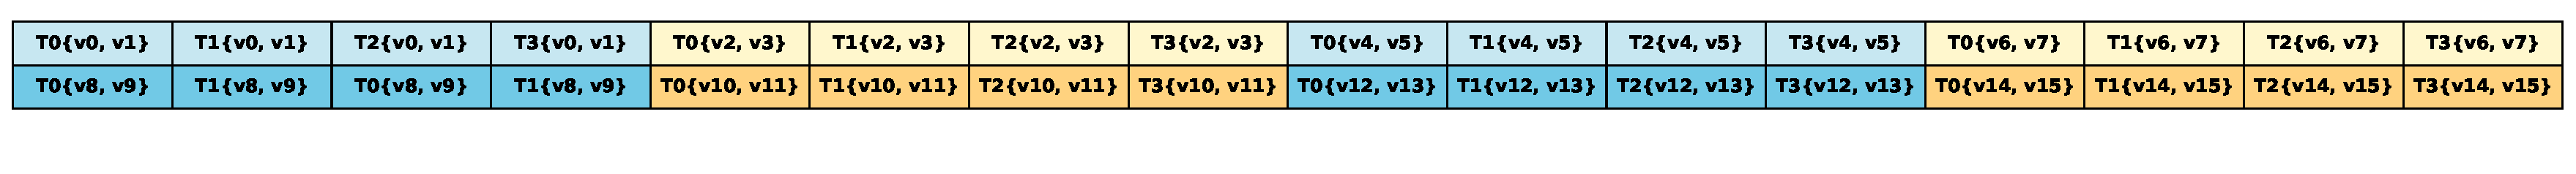
\includegraphics[width=1\columnwidth]{src/figs/new_fp32.pdf} 
    \vspace{-1em}
    \caption{Permuted \texttt{FP32} accumulator register layout - rows 0 and 8, thread 0-3, entries 0-15.}
    \label{fig:new_fp32_layout} 
\end{figure}



\subsection{Additional Experiments of using \texttt{SageBwd}}  \label{sec:appendix_exp}
Table~\ref{tab:seed_1.5b_1}--\ref{tab:seed_llama_2} show \qwen(1.5B), \qwen(3B), and \llamal(3B) fine-tuning results on four datasets with five different random seeds. The average and standard deviation show \texttt{SageBwd} is highly consistent with \texttt{BF16} across various random seeds.

\begin{table}[H]
\centering
\caption{Comparison of \texttt{SageBwd} and \texttt{BF16} performance on GSM8K and DROP across different seeds on \qwen(1.5B).}
\label{tab:seed_1.5b_1}
\scalebox{0.98}{
\begin{tabular}{cccccc}
\toprule
\multirow{2}{*}{Seed} & \multicolumn{2}{c}{GSM8K} & \multicolumn{2}{c}{DROP} \\
\cmidrule(lr){2-3} \cmidrule(lr){4-5}
& \texttt{SageBwd} & \texttt{BF16} & \texttt{SageBwd} & \texttt{BF16} \\
\midrule
\num{42}   & \num{0.5133} & \num{0.5125} & \num{0.7316} & \num{0.7364} \\
\num{233}  & \num{0.5027} & \num{0.5042} & \num{0.7269} & \num{0.7295} \\
\num{1234} & \num{0.4973} & \num{0.4973} & \num{0.7329} & \num{0.7342} \\
\num{5678} & \num{0.5201} & \num{0.5208} & \num{0.7340} & \num{0.7332} \\
\num{1}    & \num{0.5049} & \num{0.5057} & \num{0.7278} & \num{0.7404} \\
\midrule
\textbf{Avg} & \num{0.5077} & \num{0.5081} & \num{0.7307} & \num{0.7348} \\
\textbf{Std} & \num{0.0090} & \num{0.0089} & \num{0.0032} & \num{0.0040} \\
\bottomrule
\end{tabular}}
\end{table}

\begin{table}[H]
\centering
\caption{Comparison of \texttt{SageBwd} and \texttt{BF16} performance on MMLU and HellaSwag across different seeds on \qwen(1.5B).}
\label{tab:seed_1.5b_2}
\scalebox{0.98}{
\begin{tabular}{cccccc}
\toprule
\multirow{2}{*}{Seed} & \multicolumn{2}{c}{MMLU} & \multicolumn{2}{c}{HellaSwag} \\
\cmidrule(lr){2-3} \cmidrule(lr){4-5}
& \texttt{SageBwd} & \texttt{BF16} & \texttt{SageBwd} & \texttt{BF16} \\
\midrule
\num{42}   & \num{0.5814} & \num{0.5873} & \num{0.9089} & \num{0.9065} \\
\num{233}  & \num{0.5746} & \num{0.5785} & \num{0.9082} & \num{0.9049} \\
\num{1234} & \num{0.5805} & \num{0.5836} & \num{0.9025} & \num{0.9047} \\
\num{5678} & \num{0.5736} & \num{0.5693} & \num{0.9112} & \num{0.9053} \\
\num{1}    & \num{0.5830} & \num{0.5823} & \num{0.9058} & \num{0.9075} \\
\midrule
\textbf{Avg} & \num{0.5786} & \num{0.5802} & \num{0.9073} & \num{0.9058} \\
\textbf{Std} & \num{0.0043} & \num{0.0069} & \num{0.0033} & \num{0.0012} \\
\bottomrule
\end{tabular}}
\end{table}

\begin{table}[H]
\centering
\caption{Comparison of \texttt{SageBwd} and \texttt{BF16} performance on GSM8K and DROP across different seeds on \qwen(3B).}
\label{tab:seed_3b_1}
\scalebox{0.98}{
\begin{tabular}{cccccc}
\toprule
\multirow{2}{*}{Seed} & \multicolumn{2}{c}{GSM8K} & \multicolumn{2}{c}{DROP} \\
\cmidrule(lr){2-3} \cmidrule(lr){4-5}
& \texttt{SageBwd} & \texttt{BF16} & \texttt{SageBwd} & \texttt{BF16} \\
\midrule
\num{42}   & \num{0.5982} & \num{0.6232} & \num{0.7800} & \num{0.7812} \\
\num{233}  & \num{0.5997} & \num{0.5974} & \num{0.7786} & \num{0.7812} \\
\num{1234} & \num{0.6156} & \num{0.6103} & \num{0.7786} & \num{0.7824} \\
\num{5678} & \num{0.6065} & \num{0.6012} & \num{0.7816} & \num{0.7853} \\
\num{1}    & \num{0.6171} & \num{0.6073} & \num{0.7813} & \num{0.7832} \\
\midrule
\textbf{Avg} & \num{0.6074} & \num{0.6079} & \num{0.7800} & \num{0.7827} \\
\textbf{Std} & \num{0.0001} & \num{0.0001} & \num{0.0000} & \num{0.0000} \\
\bottomrule
\end{tabular}}
\end{table}

\begin{table}[H]
\centering
\caption{Comparison of \texttt{SageBwd} and \texttt{BF16} performance on MMLU and HellaSwag across different seeds on \qwen(3B).}
\label{tab:seed_3b_2}
\scalebox{0.98}{
\begin{tabular}{cccccc}
\toprule
\multirow{2}{*}{Seed} & \multicolumn{2}{c}{MMLU} & \multicolumn{2}{c}{HellaSwag} \\
\cmidrule(lr){2-3} \cmidrule(lr){4-5}
& \texttt{SageBwd} & \texttt{BF16} & \texttt{SageBwd} & \texttt{BF16} \\
\midrule
\num{42}   & \num{0.6434} & \num{0.6425} & \num{0.9419} & \num{0.9402} \\
\num{233}  & \num{0.6431} & \num{0.6437} & \num{0.9405} & \num{0.9402} \\
\num{1234} & \num{0.6492} & \num{0.6492} & \num{0.9414} & \num{0.9429} \\
\num{5678} & \num{0.6531} & \num{0.6400} & \num{0.9430} & \num{0.9440} \\
\num{1}    & \num{0.6510} & \num{0.6454} & \num{0.9446} & \num{0.9434} \\
\midrule
\textbf{Avg} & \num{0.6480} & \num{0.6442} & \num{0.9423} & \num{0.9421} \\
\textbf{Std} & \num{0.0000} & \num{0.0000} & \num{0.0000} & \num{0.0000} \\
\bottomrule
\end{tabular}}
\end{table}

\begin{table}[H]
\centering
\caption{Comparison of \texttt{SageBwd} and \texttt{BF16} performance on GSM8K and DROP across different seeds on \llamal(1B).}
\label{tab:seed_llama_1}
\scalebox{0.98}{
\begin{tabular}{cccccc}
\toprule
\multirow{2}{*}{Seed} & \multicolumn{2}{c}{GSM8K} & \multicolumn{2}{c}{DROP} \\
\cmidrule(lr){2-3} \cmidrule(lr){4-5}
& \texttt{SageBwd} & \texttt{BF16} & \texttt{SageBwd} & \texttt{BF16} \\
\midrule
\num{42}   & \num{0.2722} & \num{0.2547} & \num{0.6367} & \num{0.6447} \\
\num{233}  & \num{0.2661} & \num{0.2570} & \num{0.6456} & \num{0.6424} \\
\num{1234} & \num{0.2616} & \num{0.2873} & \num{0.6439} & \num{0.6352} \\
\num{5678} & \num{0.2684} & \num{0.2585} & \num{0.6372} & \num{0.6409} \\
\num{1}    & \num{0.2646} & \num{0.2335} & \num{0.6393} & \num{0.6441} \\
\midrule
\textbf{Avg} & \num{0.2666} & \num{0.2582} & \num{0.6405} & \num{0.6414} \\
\textbf{Std} & \num{0.0000} & \num{0.0003} & \num{0.0000} & \num{0.0000} \\
\bottomrule
\end{tabular}}
\end{table}

\begin{table}[H]
\centering
\caption{Comparison of \texttt{SageBwd} and \texttt{BF16} performance on MMLU and HellaSwag across different seeds on \llamal(3B).}
\label{tab:seed_llama_2}
\scalebox{0.98}{
\begin{tabular}{cccccc}
\toprule
\multirow{2}{*}{Seed} & \multicolumn{2}{c}{MMLU} & \multicolumn{2}{c}{HellaSwag} \\
\cmidrule(lr){2-3} \cmidrule(lr){4-5}
& \texttt{SageBwd} & \texttt{BF16} & \texttt{SageBwd} & \texttt{BF16} \\
\midrule
\num{42}   & \num{0.4665} & \num{0.4705} & \num{0.8230} & \num{0.8319} \\
\num{233}  & \num{0.4646} & \num{0.4560} & \num{0.8327} & \num{0.8256} \\
\num{1234} & \num{0.4702} & \num{0.4757} & \num{0.8202} & \num{0.8243} \\
\num{5678} & \num{0.4580} & \num{0.4639} & \num{0.8232} & \num{0.8276} \\
\num{1}    & \num{0.4666} & \num{0.4691} & \num{0.8218} & \num{0.8236} \\
\midrule
\textbf{Avg} & \num{0.4652} & \num{0.4670} & \num{0.8242} & \num{0.8266} \\
\textbf{Std} & \num{0.0000} & \num{0.0000} & \num{0.0000} & \num{0.0000} \\
\bottomrule
\end{tabular}}
\end{table}


\subsection{Transposing $V$.}  \label{sec:appendix_others}

Performing the forward propagation of attention in full \texttt{FP4} precision poses additional challenges compared to \texttt{FP16}.
The input tensors $Q$, $K$, and $V$ are typically contiguous in the head dimensions. However, the row-major constraints on \texttt{FP4} MMA for the second GEMM necessitate $V$ to be contiguous in the sequence length dimension. Calling a standalone pre-processing transpose kernel for this purpose incurs excessive overhead, particularly during inference, which is often a memory-bound situation.
We address the problem by kernel fusion. For the first problem, we fuse the transpose of $V$ into the quantization kernel, thereby avoiding additional I/O overhead. 

\subsection{Accmulated Quantization Error Analysis.} 

\begin{table}[H]
\sisetup{detect-weight=true, detect-family=true}
\centering
\vspace{-.5em}
\caption{Layer-wise L1 error analysis of \texttt{SageAttention3} on \texttt{CogVideoX-2B}. 
The second row shows the results by retaining the three most sensitive layers in \texttt{FP16}.}
\label{tab:drift_analysis}
\scalebox{0.95}{
\begin{tabular}{@{}lcccc@{}}
\toprule
\textbf{Method} & \textbf{Layer1} $\downarrow$ & \textbf{Layer10} $\downarrow$ & \textbf{Layer20} $\downarrow$ & \textbf{Layer30} $\downarrow$ \\
\midrule
Use \texttt{SageAttention3} directly & 0.0076 & 0.0922 & 0.1146 & 0.0571 \\
Keep 3 most sensitive layers in \texttt{FP16} & 0.0076 & \textbf{0.0447} & \textbf{0.0773} & \textbf{0.0429} \\
\bottomrule
\end{tabular}}
\end{table}

To explore the issue of accumulated quantization error across layers, we conduct an analysis using \texttt{SageAttention3} on \texttt{CogVideoX-2B} and report the per-layer L1 error in Table \ref{tab:drift_analysis}. We observe that the accumulated error generally increases with layer depth, though it occasionally decreases in deeper layers, suggesting partial error cancellation.
To mitigate this drift, we apply a simple yet effective strategy: keeping the three layers with the largest observed error growth in \texttt{FP16} precision. As shown in the table, this adjustment significantly reduces the overall error accumulation across layers.

\subsection{Ablation of Smoothing Techniques.}

\begin{table}[H]
\sisetup{detect-weight=true, detect-family=true}
\centering
\vspace{-.5em}
\caption{Ablation of attention accuracy with different smoothing methods on \texttt{CogVideoX-2B}. 
Smoothing K and Smoothing Q are techniques from \texttt{SageAttention} and \texttt{SageAttention2}.
}
\label{tab:smooth_ablation}
\scalebox{0.95}{
\begin{tabular}{@{}lccc@{}}
\toprule
\textbf{Method} & \textbf{Cossim} $\uparrow$ & \textbf{L1 Error} $\downarrow$ & \textbf{RMSE} $\downarrow$ \\
\midrule
None & 0.915642 & 0.335867 & 0.303483 \\
SmoothQuant & 0.930125 & 0.267617 & 0.252883 \\
Hadamard & 0.941222 & 0.262047 & 0.223970 \\
\textbf{Smoothing\_Q} & \textbf{0.982848} & \textbf{0.115658} & \textbf{0.125862} \\
\textbf{Smoothing\_K} & \textbf{0.991176} & \textbf{0.094832} & \textbf{0.097668} \\
\bottomrule
\end{tabular}}
\end{table}

To investigate the impact of different smoothing strategies on attention accuracy, we compare several existing techniques, including SmoothQuant~\citep{xiao2023smoothquant} and Hadamard transformations, which provide per-token or per-tensor scaling control. However, we find these methods less effective in our setting.
\texttt{SageAttention3} inherits the smoothing Q and smoothing K mechanisms introduced in \texttt{SageAttention2}.
We conduct an ablation study on all layers of \texttt{CogVideoX-2B} to evaluate their effects.
As shown in Table~\ref{tab:smooth_ablation}, both smoothing Q and smoothing K yield substantially higher cosine similarity and lower reconstruction errors, demonstrating their effectiveness in stabilizing quantized attention computation.


\subsection{Theoretical Speed Comparison.} 

\begin{table}[H]
\sisetup{detect-weight=true, detect-family=true}
\centering
\vspace{-.5em}
\caption{Theoretical throughput comparison between FlashAttention3 and \texttt{SageAttention3} across different GPUs.}
\label{tab:theoretical_tops}
\scalebox{0.95}{
\begin{tabular}{@{}lccc@{}}
\toprule
\textbf{Method} & \textbf{B300 TOPS} $\uparrow$ & \textbf{B200 TOPS} $\uparrow$ & \textbf{RTX5090 TOPS} $\uparrow$ \\
\midrule
FlashAttention3 & 2500 & 2500 & 209.5 \\
FlashAttenion3 (\texttt{FP8}) & 5000 & 5000 & 419 \\
\textbf{\texttt{SageAttention3 (FP4)}} & \textbf{15000} & \textbf{10000} & \textbf{1676} \\
\bottomrule
\end{tabular}}
\end{table}

To provide a theoretical comparison with FlashAttention3, we refer to NVIDIA’s official documentation on throughput (TOPS) across different precisions. Since FlashAttention3 is currently only supported on \texttt{H100} GPUs, a direct empirical comparison is not feasible. Instead, we estimate the theoretical compute throughput of both FlashAttention3 and our \texttt{SageAttention3} on GPUs that support \texttt{FP4} Tensor Cores (\texttt{B300}, \texttt{B200}, and \texttt{RTX5090}).
As summarized in Table~\ref{tab:theoretical_tops}, \texttt{SageAttention3} achieves substantially higher theoretical peak throughput, highlighting its potential for further accelerating attention computation beyond FlashAttention-3.

\subsection{FlashAttentions vs SageAttentions.}

\begin{table}[H]
\sisetup{detect-weight=true, detect-family=true}
\centering
\vspace{-.5em}
\caption{Speed–accuracy trade-off of different attention methods.}
\label{tab:tradeoff}
\scalebox{0.95}{
\begin{tabular}{@{}lccc@{}}
\toprule
\textbf{Method} & \textbf{TOPS on 5090} $\uparrow$ & \textbf{TOPS on H100} $\uparrow$ & \textbf{Accuracy (CosSim)} $\uparrow$ \\
\midrule
FlashAttention2 & 214 & 338 & 100.000\% \\
FlashAttention3 (16bit) & N/A & 470 & 100.000\% \\
FlashAttention3 (8bit) & N/A & 890 & 98.570\% \\
SageAttention1 & 479 & 518 & 99.996\% \\
SageAttention2 (8bit) & 643 & 885 & 99.995\% \\
\texttt{SageAttention3 (4bit)} & \textbf{1038} & N/A & \textbf{99.551\%} \\
\bottomrule
\end{tabular}}
\label{tab:h100_5090_speed}
\end{table}

To illustrate the trade-off between accuracy and speed, we recorded the accuracy (Cosine similarity) of various attention methods across all layers of \texttt{CogVideoX-2B}, along with their theoretical throughput on \texttt{RTX5090} and \texttt{H100} GPUs. These results are summarized in the Table~\ref{tab:h100_5090_speed}.


% \begin{table}[h]
% \centering
% \caption{L1 Error of $Q$, $K$, and $V$ gradients.}
% \begin{tabular}{lccc}
% \toprule
% Method & $dQ$ L1 Error $\downarrow$ & $dK$ L1 Error $\downarrow$ & $dV$ L1 Error $\downarrow$ \\
% \midrule
% INT8 SageBwd & \textbf{0.0290} & \textbf{0.0317} & \textbf{0.0423} \\
% FP8 SageBwd & 0.0696 & 0.0999 & 0.0873 \\
% \bottomrule
% \end{tabular}
% \end{table}

% \begin{table}[h]
% \centering
% \caption{Cosine similarity of $Q$, $K$, and $V$ gradients.}
% \begin{tabular}{lccc}
% \toprule
% Method & $dQ$ CosSim $\uparrow$ & $dK$ CosSim $\uparrow$ & $dV$ CosSim $\uparrow$ \\
% \midrule
% INT8 SageBwd & \textbf{0.9987} & \textbf{0.9993} & \textbf{0.9995} \\
% FP8 SageBwd & 0.9880 & 0.9910 & 0.9955 \\
% \bottomrule
% \end{tabular}
% \end{table}

\subsection{Analysis of Two-Level Quantization.} 
\begin{proof}

We analyze the relative quantization error of $\widetilde \vP$ using both \texttt{direct quantization} and \texttt{two-level quantization} as follows:

For \texttt{direct quantization}, the relative quantization error, denoted as $E_1$, is defined as:
\begin{align}
    %\widetilde \vP =& \texttt{OnlineSoftmax}(\vS)  \notag \\
    \mathbf{s_P}, \hat \vP = \phi(\widetilde \vP), ~~~ E_1 = \frac{|\mathbf{s_P} \times \hat \vP - \widetilde \vP|}{|\widetilde \vP|}
    \label{err_1}
\end{align}


%(2) Two-level quantization:
%\begin{align*}
%    E_2 =  |\hat \vP_2 \times \mathbf{s_{P_2}} \times \mathbf{s_{P_1}} - \widetilde \vP|
%    = |\hat \vP_2 \times \mathbf{s_{P_2}}|
%\end{align*}

%The first-level quantization in two-level quantization is as follows:
For \texttt{two-level quantization}, the first level proceeds as:
\begin{align*}
    \mathbf{s_{P_1}} = \rowmax(\widetilde \vP) / (448 \times 6), ~~~
     \widetilde \vP_2 &= \widetilde \vP / \mathbf{s_{P_1}}, ~~~
\end{align*}

The quantization error introduced in this first step is negligible because $\widetilde \vP$, $\widetilde\vP_2$, and $s_{P_1}$ are all represented in \texttt{FP32} format.

We focus primarily on the second-level quantization, where the relative quantization error $E_2$ is given by:
\begin{align}
     \mathbf{s_{P_2}}, \hat \vP_2 = \phi (\widetilde \vP_2),~~~
     E_2 = \frac{|\mathbf{s_{p_2}} \times \hat \vP_2 - \widetilde \vP_2|}{|\widetilde \vP_2|}
     \label{err_2}
\end{align}

% The final error of two-level quantization is:
% \begin{align*}
%     E_{two-level} = E_2 / \mathbf{s_{P_1}}
% \end{align*}

The key difference between Equation~\ref{err_1} and \ref{err_2} lies in the range of the \texttt{FP8} scale factor.

Let $\{X\}_n$ denote the number of distinct representable values in the set $X$. Then:

in \texttt{direct quantization}:
\begin{align*}
    0 \le \mathbf{s_{P}} \le 0.167,~~~ \mathbf{s_{P}} \in \mathbf{E4M3}, ~~~ \{\mathbf{s_{P}}\}_n = 35
\end{align*}

In \texttt{two-level quantization}:
\begin{align*}
    0 \le \mathbf{s_{P_2}} \le 448.0, ~~~ \mathbf{s_{P_2}} \in \mathbf{E4M3}, ~~~ \{\mathbf{s_{P_2}}\}_n = 127
\end{align*}

Since $\{\textbf{E2M1}\}_n = 8$, the number of unique outputs after dequantization is:

For \texttt{direct quantization}:
\begin{align*}
    \widetilde \vP^{\prime} = \mathbf{s_{P}} \times \hat \vP, ~~~ \{\widetilde \vP^{\prime} \}_n = 35 \times 8 = 280
\end{align*}

For \texttt{two-level quantization}:
\begin{align*}
    \widetilde \vP_{2}^{\prime} = \mathbf{s_{P_2}} \times \hat \vP_2, ~~~ \{\widetilde \vP_2^{\prime} \}_n = 127 \times 8 = 1016
\end{align*}

Let $\Delta(p_i)$ denote the interval between the two nearest quantization levels surrounding the value $p_i \in \widetilde \vP$.
Then the absolute quantization error satisfies:
%interval between two neighbour quantization candidate values, We have:
\begin{align*}
|\hat p_i - p_i| \le \frac{\Delta(p_i)}{2}
\end{align*}
The relative error $\varepsilon$ satisfies:
\begin{align*}
   \varepsilon_i \le \frac{\Delta(p_i)}{2 \times p_i}
\end{align*}

Given that $\{\widetilde \vP_2^{\prime} \}_n > \{\widetilde \vP^{\prime} \}_n$, the quantization intervals in the two-level scheme are finer:
\begin{align*}
\frac{\Delta(\widetilde \vP_2)}{\widetilde \vP_2} < \frac{\Delta(\widetilde \vP)}{\widetilde \vP}
\end{align*}

%Thus, we have the upper bound relative error of two quantization strategy:
Thus, the relative quantization error satisfies:
\begin{align*}
\frac{|\widetilde \vP_2^{\prime} - \widetilde \vP_2|}{\widetilde \vP_2} <  \frac{|\vP^{\prime} - \widetilde \vP|}{\widetilde \vP} 
\end{align*}

Which leads to the conclusion:
\begin{align*}
    E_2 < E_1
\end{align*}
%Finished the proof.

\end{proof}


% To make the $E_1$ in Equation \ref{err_1} and Equation \ref{err_2} in the same magnitude, we can do as follows:
% \begin{align*}
%     E_1^{*} = |\mathbf{s_P} \times \hat \vP - \widetilde \vP| \times \frac{1}{\mathbf{s_{P_1}}}
% \end{align*}






%the scale factor $s_{P}$ ranging from 0 to about 0.167 in E4M3 format,



\subsection{Analysis of the Benefit of Keeping $\vdO_i\vV_j^\top$ in FP16 in \texttt{SageBwd}.}

The backward pass of \texttt{SageBwd} involves 5 MatMuls. The accuracy of $\vS_{ij}=\vQ_i\vK_j^\top$ is fully addressed in SageAttention2. The remaining four are as follows:

\begin{enumerate}
    \item[(1)] $\vdP_{ij}=\vdO_i\vV_j^\top$.
    \item[(2)] $\vdQ_i\gets\vdQ_i+\vdS_{ij}\vK_j$
    \item[(3)] $\vdK_j\gets\vdK_j+\vdS_{ij}^\top\vQ_i$
    \item[(4)] $\vdV_j\gets\vdV_j+\vP_{ij}^\top\vdO_i$
\end{enumerate}

We choose to keep (1) in FP16, while quantizing others to INT8. This choice can be formally justified:

\begin{proof}
Following~\citep{lin2023awq}, we assume that any matrix ${\bf X}\in\mathbb R^{n\times d}$ (e.g. $\vQ,\vK,\vV,\vdO$) satisfies:

\begin{itemize}
    \item The entries in $\bf X$ are mutually independent.
    \item ${\bf X}_{ij} \sim N(\mu_{{\bf X},j},\sigma_{{\bf X},j}^2)$, i.e. the distribution of each token is identical.
\end{itemize}

The quantization error of a matrix $\bf X$ is denoted as:
$$
\Delta{\bf X}:=s_{\bf X}\hat{\bf X} - {\bf X},\quad \text{where }s_{\bf X},\hat{\bf X} = \psi({\bf X}).
$$

For example, consider the error in $\vdQ$. Neglecting second-order error terms, we have:
$$
\Delta\vdQ = \underbrace{(\vP \circ (\vdO\Delta\vV^\top + \Delta \vdO\vV^\top))\vK}_{\Delta\vdQ^{(1)} \text{ from (1)}} + \underbrace{\Delta \vdS \vK + \vdS \Delta \vK}_{\vdQ^{(2)}\text{from (2)}}.
$$

Here, $\vdS=\vP\circ(\vdP-D)=\vP\circ(\vdO\vV^\top-D)$, where $D=\vdO\odot\vO$. In element-wise terms (the subscript denotes a single element):
$$
\vdS_{ij} = \vP_{ij} \sum_k \vdO_{ik} (\vV_{jk} - \vO_{ik}) = \vP_{ij}\sum_k \vdO_{ik}\left(\vV_{jk} - \sum_\ell \vP_{i\ell}\vV_{\ell k}\right)
$$

Since $\vV$ is independent of other variables, by linearity of expectation:
$$
\mathbb E[\vdS_{ij}] = \mathbb E\left[\vP_{ij}\sum_k\vdO_{ik}\left(\mu_{\vV,k}-\sum_\ell\vP_{i\ell} \mu_{\vV,k}\right)\right] = 0.
$$

Moreover, as negating $\vV$ flips the sign of $\vdS_{ij}$, the PDF of $\vdS_{ij}$ is symmetric. Using a "round-to-nearest" quantization policy, we have $\mathbb E[\Delta\vdS]=0$. Thus
$$
\mathbb E\left[\vdQ^{(2)}\right] = \mathbb E[\Delta\vdS\vK + \vdS\Delta\vK] = 0,
$$

while $\mathbb E\left[\Delta\vdQ^{(1)}\right]$ is generally non-zero (e.g. when distributions have non-zero means), indicating that $\vdQ$'s error is dominated by $\Delta\vdQ^{(1)}$.

\end{proof}



\subsection{Broader Impact}
This paper presents work that aims to advance the field of efficient machine learning systems. It can be used to accelerate the inference and training processes of various models. None of the negative impacts we feel must be specifically highlighted here.